\section{Systembeskrivelse}
Der ønskes, som tidligere nævnt, at udvikle et system, der har til formål at støtte musklerne omkring knæleddet hos ALS-patienter under udførelse af en squat-øvelse. Dette gøres for at aflaste patienterne med henblik på at kunne undgå kørestol i tidlige stadier af ALS. Systemet skal kunne opsamle EMG-signaler fra rectus femoris og vinklen over knæleddet. Disse signaler skal behandles således, at de kan omsættes til signaler, så en prototype af et exoskelet kan udføre en tilsvarende bevægelse. Systemet har også som mål, at det skal have mulighed for forstærkning af signalet, så mindre muskelkraft også vil kunne udløse den samme bevægelse af knæleddet. Derudover skal systemet være brugervenligt ved at være kompakt, mobilt og ikke generende over for brugeren.

\subsection{Krav til systemet} 
\begin{itemize}
\item Systemet skal registrere muskelaktivitet af rectus femoris og vinklen i knæleddet
\item Systemet skal kunne overføre data trådløst til en computer
\item Systemet skal kunne ende ud i en prototype af et exoskelet
\item Systemet skal være batteridrevet
\item Systemet skal være sikkert og ikke til gene for brugeren 
\item Systemet skal kunne indikere, hvis der ikke er strøm nok til at virke optimalt
\end{itemize}


\subsection{Blokdiagram}
\begin{figure}[H]
\centering
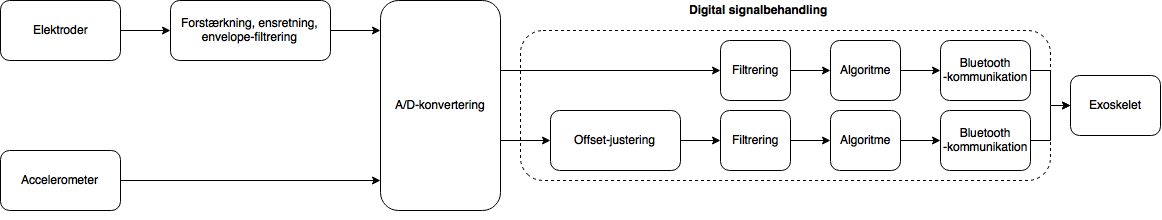
\includegraphics[width=1\textwidth]{figures/blokdiagram.png}
\caption{Systemets opbygning.}
\label{fig:blokdiagram}
\end{figure}

I dette projekt er der valgt at udarbejde en prototype, som har til formål at bøje knæleddet, når rectus femoris kontraherer. Opbygningen af systemet fremgår af \autoref{fig:blokdiagram}. Der anvendes to sensorer, EMG-elekroder og accelerometre, til at opsamle biologiske signaler. For at registrere muskelaktivitet anvendes elektroder og en EMG-forstærker, der har til formål at forstærke, filtrere og ensrette muskelsignalet, der opsamles. Accelerometre anvendes for at give systemet et input om, knæleddets vinkling  under en squat-øvelse. Det opsamlede signal sendes herefter videre til den digitale del af systemet, hvilket er bestående af et Bluetooth Low Energy Pioneer kit (CY8CKIT-042-BLE), som opfanger de biologiske signaler og overfører dem trådløst til en CySmartUSB BLE Dongle sat i en computer, som kan kommunikere med prototypen af exoskelettet udarbejdet i LEGO Mindstorm \fxnote{tjek om dette er rigtigt}. 


